

\begin{figure}[h]
	\centering
	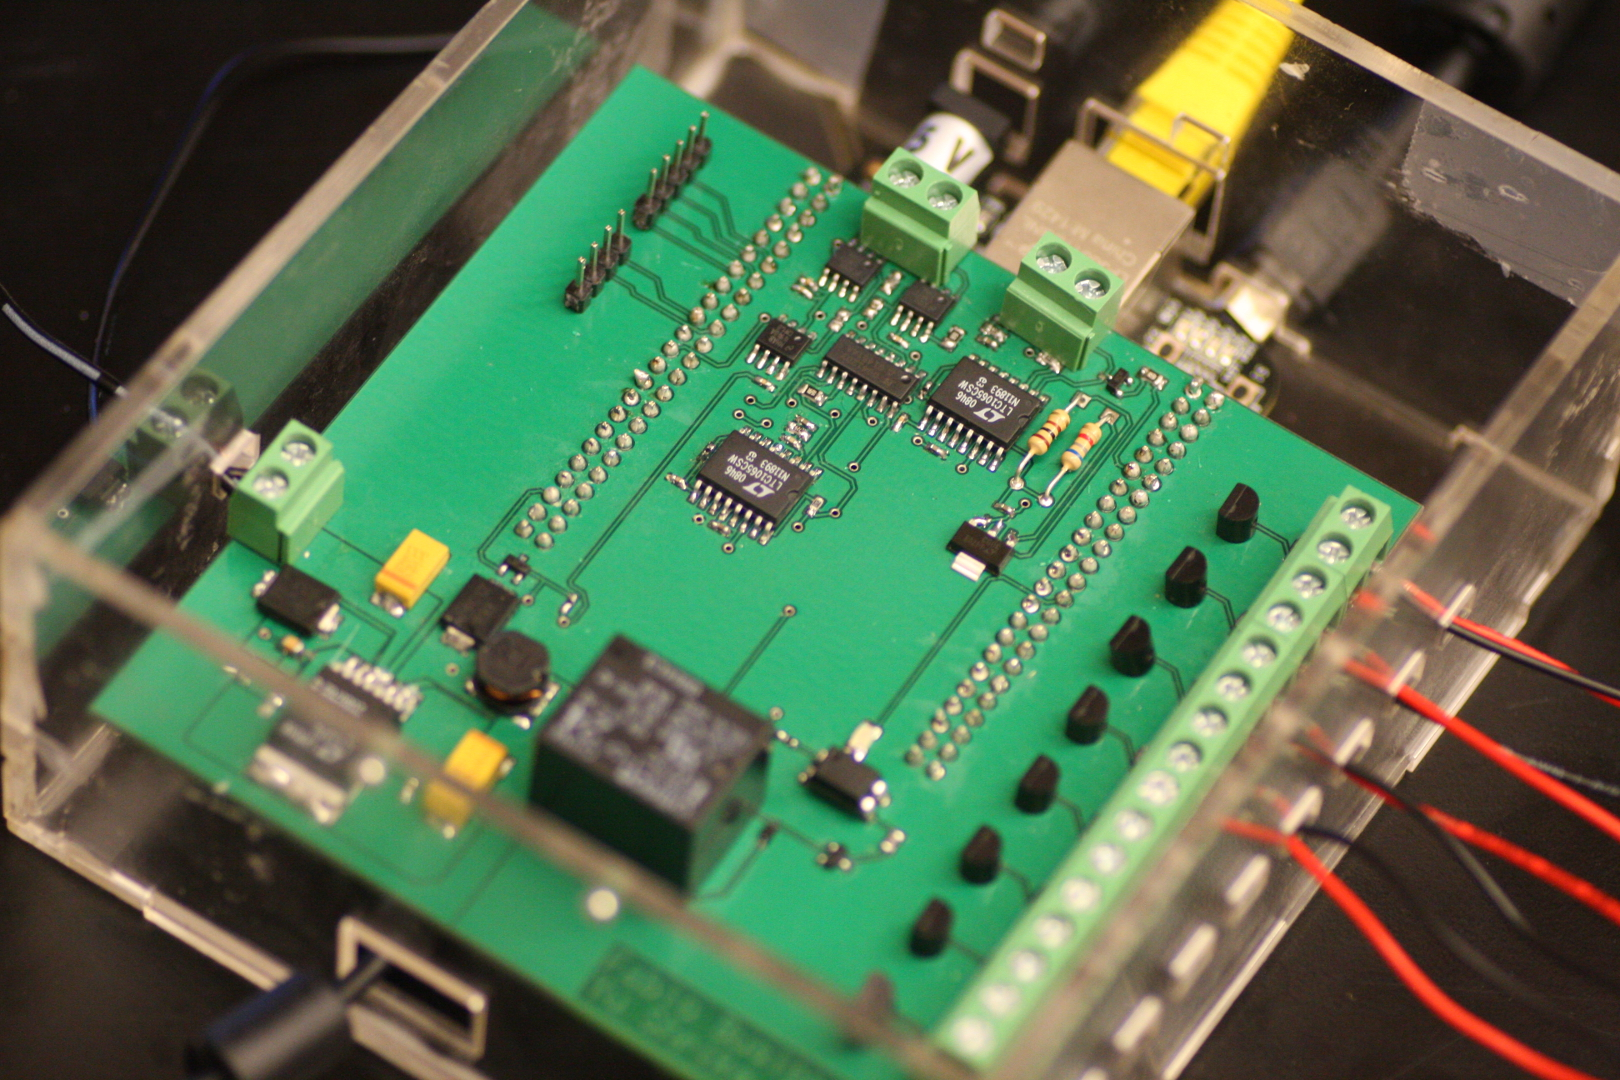
\includegraphics[width = \textwidth]{circuitfinisched}
	\caption{Final system mounted on a PCB}
	\label{Fig:finalcircuit}
\end{figure}


All the hardware and the circuit described so far has been mounted on a Printed Circuit Board (\textit{PCB}) that is supposed to be a \textit{cape} of the Beaglebone Black. This means that the whole physical structure has been made to be attached on the headers of the board. In (Fig.\ref{Fig:circuit}) all the circuit that has to be made on the \textit{PCB} is shown.\\

The PCB has been designed in a two-layer board ($100\ x\ 100\ mm$) using the \textit{National Instruments Circuit Design Suite},  in particular \textit{Multisim} to carry out the schematic and \textit{Ultiboard} for what concern the PCB.\\
The design has followed the guidelines for reduced electromagnetic interface (\textit{EMI}). First of all, since Surface-mount devices (\textit{SMD}) are better than Through-hole components (\textit{THD}) in dealing with RF energy, because of reduced inductances and closer component placements available (\cite{PDGFRE}), where there was a choice, \textit{SMD} components have been used. \\

Particular attention has been paid for the \textit{DC-DC} converter layout, because a wrong \textit{PCB} design for switching power supply often means failure. Moreover, in these terms, what is good for \textit{EMI} is also good in terms of functional stability for the regulator.\\




\begin{figure}[t]
	\begin{center}
	\includegraphics[angle = 90, width = \textwidth]{pcb/circuit1}
	\caption{Schematic of Complete Circuit}
	\label{Fig:circuit}
	\end{center}
	
	
\end{figure}

 \clearpage
 
 The circuit in (Fig.\ref{Fig:High}) is schematically a common buck regulator. In that figure, with a blue circle, is highlighted the high speed switching current path: the loop which produces the highest \textit{EMI}. Indeed, in  the blue loop flows a fully switched alternated current, and for this reason it is also referred as \textbf{hot loop}.

\begin{figure}[h]
	\centering
	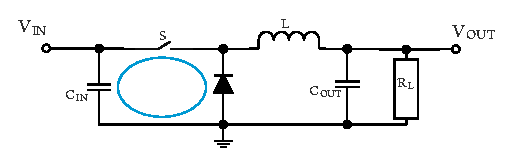
\includegraphics[width = \textwidth]{pcb/dcdcloop}
	\caption{\textit{DC-DC} High Speed Switching Path}
	\label{Fig:High}
\end{figure}

In order to ensure clean switching and reduce \textit{EMI} the minimum lead length is required for reducing the radiating effect of the hot loop as much as possible: and so it has been done, as can be seen from (Fig.\ref{Fig:dcdc-pcb}).

\begin{figure}[h]
	\centering
	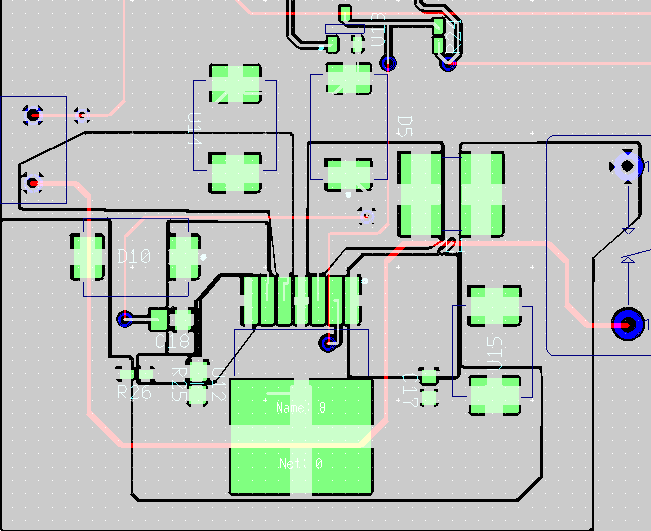
\includegraphics[width = \textwidth]{pcb/dcdc-pcb1}
	\caption{\textit{PCB} Layout of \textit{DC-DC}}
	\label{Fig:dcdc-pcb}
\end{figure}

In (Fig.\ref{Fig:dcdc-pcb}) the \textit{PCB} layout for \textit{DC-DC} converter has been shown, in which we can see that: 
\begin{itemize}
	\item the magnetic radiation is minimized by keeping by keeping catch diode and the input capacitor leads as short as possible;
	\item the electric radiation is minimized by reducing the area and length of all traces connected to the switch and boost pins.
\end{itemize}

Moreover, in order to reduce the noise on the feedback, that is translated in error on output voltage, the switch node and the feedback resistors are kept as far as possible from each others.\\

The (Fig.\ref{fig:PCB}) shows the \textit{PCB} layout without ground plane (Fig.\ref{subfig-1:pcb}), then with both top and bottom ground plane (Fig.\ref{subfig-2:pcbboth}) which help with heat dissipation and \textit{EMI} reduction. In (Fig.\ref{subfig-2:pcb3d}) and (Fig.\ref{subfig-2:pcbphoto}) the 3-D model generated using \textit{Ultiboard} and the final real result are compared.


\begin{figure}[h]
	\subfloat[\textit{PCB} Layout Withot Ground Plane\label{subfig-1:pcb}]{%
		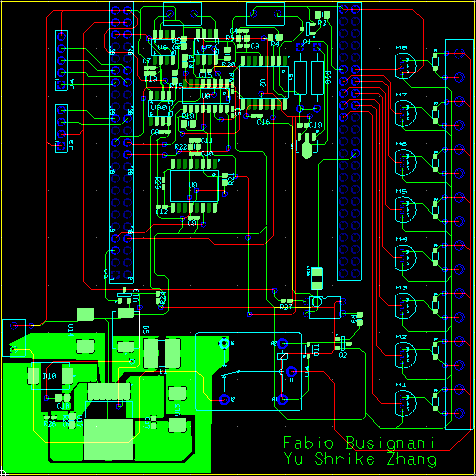
\includegraphics[width=.5\textwidth]{pcb/PCB}
	}
	\subfloat[\textit{PCB} Layout With Both Top and Bottom Ground Plane\label{subfig-2:pcbboth}]{%
		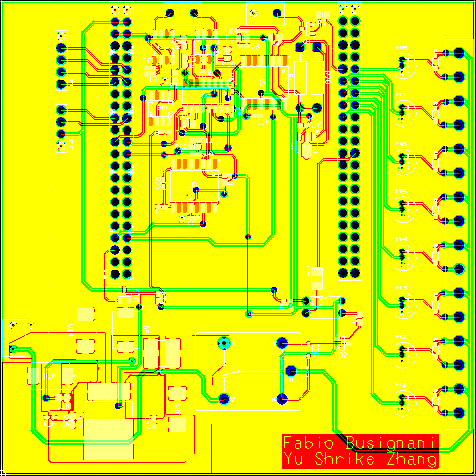
\includegraphics[width=.5\textwidth]{pcb/PCB-both}
	}\\
	\subfloat[\textit{PCB} 3-D Model View\label{subfig-2:pcb3d}]{%
		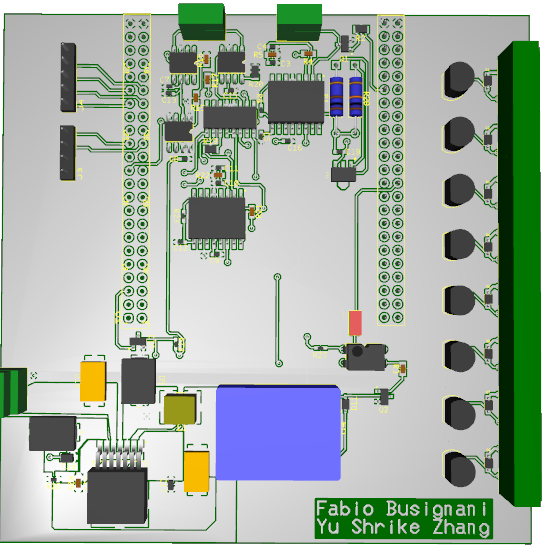
\includegraphics[width=.5\textwidth]{pcb/pcb-up}
	}
	\subfloat[\textit{PCB} Real Result\label{subfig-2:pcbphoto}]{%
		\includegraphics[width=.5\textwidth]{pcb/foto}
	}
	\caption{PCB of the System}\label{fig:PCB}
\end{figure}
